\lab{Gaussian Mixture Models}{Gaussian Mixture Models}
\objective{Understand the formulation of Gaussian Mixture Models (GMMs) and use the Expectation Maximization algorithm to estimate GMM parameters.}


% I really don't like this old explanation
\begin{comment}
You've already seen GMMs as the observation distribution in certain continuous density HMMs. Here, we will discuss them further and learn how to estimate their parameters, given data.

The main idea behind a mixture model is contained in the name, i.e. it is a \emph{mixture} of different models. What do we mean by a mixture? A mixture model is composed of $K$ \emph{components}, each component being responsible for a portion of the data. The responsibilities of these components are represented by mixture \emph{weights} $w_{i}$, for $i = 1, \cdots, k$. As you may have guessed, these weights are nonnegative and sum to $1$. Thus component $j$ is responsible for $100\cdot w_{j}$ percent of the data generated by the model.

Each component is itself a probability distribution. In a GMM, each component is specifically a Gaussian (multivariate normal) distribution. Thus we additionally have parameters $\mu_{i}, \Sigma_{i}$ for $i = 1, \cdots, K$, i.e. a mean and covariance for each component in the GMM. It is important here to keep in mind that a GMM does not arise from adding weighted multivariate normal random variables, but rather from weighting the responsibility of each multivariate normal random variable. In the first case, we would simply have a different multivariate normal distribution, whereas in the second case we have a mixture. Refer to Figure \ref{fig:gmm-threedplots} for a visualization of this.
\end{comment}

\begin{comment}
%this example is based on one in the volume 3 book
Suppose we have two seemingly-identical coins.
One of these coins is fair, with a probability \(p=0.5\) of landing as heads, while the other coin is biased, with probability \(p=0.7\) of landing as heads.
We perform an experiment by randomly selecting one of the coins, flipping that coin 5 times, and letting \(X\) be the number of heads.
This leads to a question: how is \(X\) distributed?
The answer is in fact \textit{not} that \(X\) is binomially-distributed; rather, \(X\) is an example of a \textit{mixture model} made from binomial distributions.
\end{comment}

Mixture models are a useful way to combine distributions together that allows us to describe much more complicated distributions than using just the standard list of named distributions.
The essential idea of a mixture model is in its name: it is a mixture of several different models, or probability distributions.
Each of these model is called a \emph{component}.
Each component has a certain probability associated with it, called its \emph{weight}, that describes how likely it is for a sample from the model to come from that component.
We denote the weight of the \(i\)-th component as \(w_i\).

In this lab, we focus on \emph{Gaussian Mixture Models}, or GMMs for short.
In a GMM, each component is a multivariate %\footnote{Strictly speaking, they can also be univariate, but the distinction is minor} 
 Gaussian (normal) distribution.
Each of these is parameterized by a mean \(\mu_i\) and a covariance matrix \(\Sigma_i\).

A GMM with \(K\) components thus has parameters \(\theta = \left(w_1,\ldots,w_K, \mu_1,\ldots,\mu_K,\Sigma_1,\ldots,\Sigma_K\right)
\).
We can use the law of total probability to evaluate the density of a GMM, which is given by 
\[
P(z | \theta) = \sum_{k=1}^{K} w_{k} \mathcal{N}(z | \mu_{k}, \Sigma_{k})
\]
where
\[
\mathcal{N}(z | \mu, \Sigma) = \frac{1}{\sqrt{\det(2\pi\Sigma)}} \exp\left({-\frac{1}{2} \left(z - \mu \right)^{T} \Sigma^{-1} \left(z - \mu\right)}\right)
\]
is the density function of a multivariate normal distribution.

It is important to keep in mind that a GMM does \emph{not} arise from adding weighted multivariate normal random variables, but rather from weighting the responsibility of each multivariate normal random variable. 
The first case simply results in a different multivariate normal distribution. %\footnote{If they are independent; if they aren't, weird things can happen.} 
Refer to Figure \ref{fig:gmm-threedplots} for a visualization of these two cases.

\begin{figure}[h]
\centering
	\begin{subfigure}[b]{.49\textwidth}
		\centering
		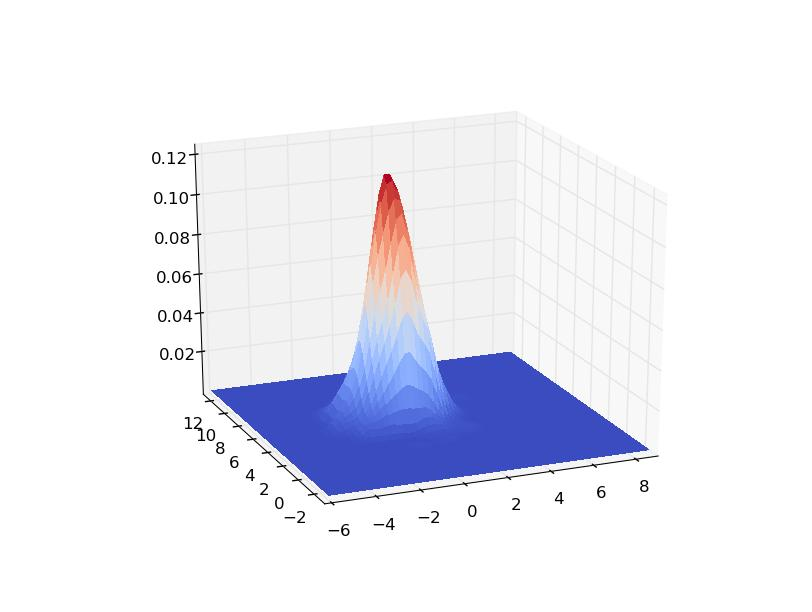
\includegraphics[width=\textwidth]{figures/sum.jpeg}
		\caption{Sum of weighted multivariate normal random variables.}
	\end{subfigure}
	\begin{subfigure}[b]{.49\textwidth}
		\centering
		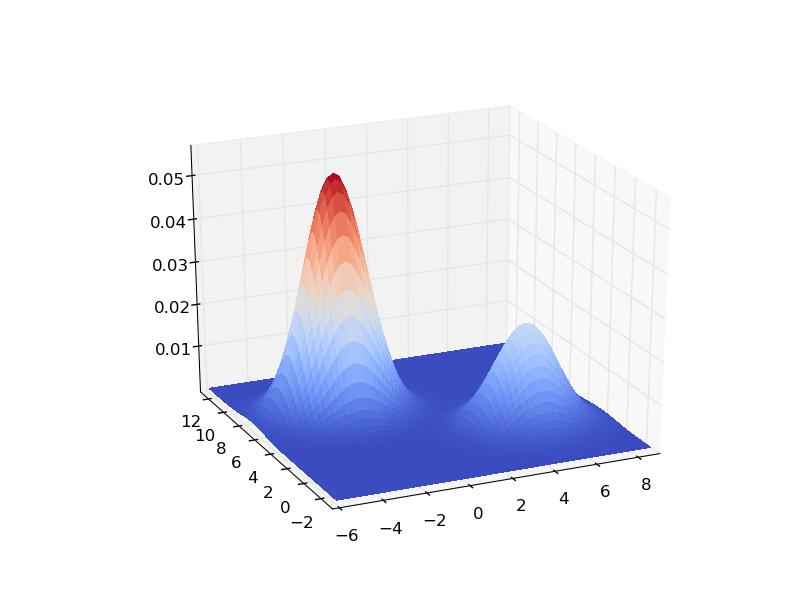
\includegraphics[width=\textwidth]{figures/gmm.jpeg}
		\caption{Weighted mixture of multivariate normal random variables.}
	\end{subfigure}
    \caption{}
	\label{fig:gmm-threedplots}
\end{figure}


% Old problems
\begin{comment}
\begin{problem}
Write a function to evaluate the density of a normal distribution at a point $x$, given parameters $\mu$ and $\Sigma$. Include the option to return the log of this probability, but be sure to do it intelligently! Also write a function that computes the density of a GMM at a point $x$, given the parameters $\lambda$, along with the log option.
\end{problem}

\begin{problem}
Write the skeleton of a GMM class. In the \li{\_\_init\_\_} method, it should accept the non-null parameter \emph{n\_components}, as well as parameters for the weights, means, and covariance matrices which define the GMM. Include a function to generate data from a fully defined GMM (you may use your code from the CDHMM lab for this), as well as the density function you recently defined.
\end{problem}
\end{comment}

\begin{problem}
Throughout this lab, we will build a GMM class with various methods.
%todo decide if this is a good idea
Write the \li{__init__} method for this class.
It should accept a parameter for the number of components and optional parameters for the weights, means, and covariance matrices which define the GMM, and store these.\footnote{
If we don't have a good guess for the parameters of the GMM to pass into the class, it makes more sense to initialize these from the dataset we are training on, which we will do later in the \lif{fit} method; hence, we let the parameters be optional here.
}

If we have \(K\) components and \(d\) dimensions, then the weights should have shape \li{(K,)}, the means \li{(K,d)}, and the covariances \li{(K,d,d)}.
The parameters for the \(k\)-th component can be found as \li{weights[k], means[k], covars[k]}.
\end{problem}
%%
\begin{problem}
Write a method \li{component_logpdf} for your class that accepts a component \li{k} and a point \li{z} and computes 
\[
\log w_k + \log \mathcal{N}(z|\mu_k,\Sigma_k)
,
\]
the logarithm of the contribution of the \(k\)-th component of the pdf.
Also write a method \li{pdf} that accepts a point \li{z} and returns the probability density of the whole GMM at that point.

Hint: \li{scipy.stats.multivariate_normal.pdf} and \li{scipy.stats.multivariate_normal.logpdf} can be used to efficiently evaluate the multivariate normal pdf.

To test your functions, create the following GMM:
\begin{lstlisting}
gmm = GMM(n_components = 2,
        weights = np.array([0.6, 0.4]),
        means = np.array([[-0.5, -4.0], [0.5, 0.5]]),
        covars = np.array([
            [[1, 0],[0, 1]],
            [[0.25, -1],[-1, 8]],
        ]))
\end{lstlisting}
Your functions should give the following output:
\begin{lstlisting}
>>> gmm.pdf(np.array([1.0, -3.5]))
0.05077912539363083
# Component 0
>>> gmm.component_logpdf(0, np.array([1.0, -3.5]))
-3.598702690175336
# Component 1
>>> gmm.component_logpdf(1, np.array([1.0, -3.5]))
-3.7541677982835004
\end{lstlisting}
Note that since this GMM is 2-dimensional, the input point must be an array of length 2.
\label{prob:gmm_has_example}
\end{problem}

In order to draw a value from a mixture model, we must first draw a variable \(X \sim \mathrm{Cat}(w_1,\ldots, w_K)\) that represents which component the sample comes from.
We can then draw the sample \(Z\sim \mathcal{N}(\mu_X, \Sigma_X)\).
If we want to draw multiple samples, we need to repeat this process for each one (draw an \(X\) and then draw a \(Z\).

\begin{problem}
Write a method \li{draw} for the GMM class that randomly draws from the model.
If \li{m} points are drawn and the GMM is \(d\)-dimensional, the returned array should have shape \li{(m,d)}.

Draw a sample of 10,000 points from the GMM defined in Problem \ref{prob:gmm_has_example}.
Plot the pdf of the GMM (using \li{plt.pcolormesh}) and a hexbin plot of the drawn points.
How do the plots compare?

The following code can be used to plot the pdf:
\begin{lstlisting}
## Create the grid to plot on
x = np.linspace(-8,8,100)
y = np.linspace(-8,8,100)
X, Y = np.meshgrid(x, y)
## Calculate the pdf at each point
# If your pdf function uses array broadcasting, you can do the following:
Z = gmm.pdf(np.dstack((X,Y)))
# Otherwise, you need to iterate over each point:
Z = np.array([[
        gmm.pdf([X[i,j], Y[i,j]]) for j in range(100)
        ] for i in range(100)
    ])
## Create the plot
plt.pcolormesh(X, Y, Z, shading='auto')
\end{lstlisting}
\label{prob:gmm_plot_example}
%Note: specifying shading='auto' is necessary in current versions of matplotlib to avoid a deprecation warning; may not be necessary in the near future.
%If you find the situation has changed, then shading='auto' may be removed safely.
\end{problem}

We now consider how to estimate the parameters of a GMM given some observed data \(Z = z_1,\ldots, z_n\).
Ordinarily, a good approach would be to try to directly maximize the log-likelihood
\[
l(\theta)=\sum_{i=1}^n\log\sum_{j=1}^Kw_{j} \mathcal{N}(z_i | \mu_{j}, \Sigma_{j}).
\]
However, this expression is very difficult to deal with using standard optimization methods, particularly because of the sum inside of the logarithm.
A good alternative in this case is the \emph{expectation maximization} (EM) algorithm.
This is an iterative algorithm, where each step consists of maximizing a function that is designed to approximate the log-likelihood while being much easier to maximize.

Each iteration consists of two steps, the E-step and the M-step.
Suppose our estimated parameters at the \(t\)-th iteration are \(\theta^t=\left(w_1^t,\ldots,w_K^t, \mu_1^t,\ldots,\mu_K^t,\Sigma_1^t,\ldots,\Sigma_K^t\right)\).
Note that \(t\) is an index, not an exponent.
For each data point \(z_i, 1\leq i \leq n\) and each component \(1\leq k\leq K\), the E-step consists of computing
\begin{align*}
q_i^t(k) &=
P(X_i=k | z_i, \theta^t)
\\
&=
\frac{P(z_i|X_i=k,\theta^t)}{P(z_i|\theta^t)}
\\
&= 
\frac{
w_k^t \,\mathcal{N}(z_i| \mu_k^t,\Sigma_k^t)
}{
\sum_{k'=1}^K
w_{k'}^t \,\mathcal{N}(z_i| \mu_{k'}^t,\Sigma_{k'}^t)
}
\end{align*}

In order to accurately compute this quantity, however, we need to be more careful.
It is possible that due to floating point underflow\footnote{As a refresher, one way that floating point numbers are limited is that they cannot represent positive numbers arbitrarily close to zero; at some point, if the number in a computation becomes too small, the computer is forced to round it to zero, which is called \emph{underflow}. The threshhold is about \(10^{-323}\) for the 64-bit floating point numbers used in python. Even if underflow does not occur, very small floating points have greatly reduced precision, so it is generally good to avoid using them.} that each term 
\(
w_{k'}^t \,\mathcal{N}(z_i| \mu_{k'},\Sigma_{k'})
\)
in the sum in the denominator becomes zero, which is a major problem.
This particularly happens if the exponents in the multivariate normal densities all are large negative numbers.
To avoid this problem, we can rescale the numerator and denominator.
Let 
\[
\ell_{i,k} = \log w_{k}^t +\log\mathcal{N}(z_i| \mu_{k}^t,\Sigma_{k}^t),\]
the logarithm of each term in the denominator.
For each data point \(z_i\), we can find
\[
L_i
=\max_{k'} \ell_{i,{k'}},
\]
the largest of these logarithms.
Then, we can rewrite the quantity we want to calculate as
\begin{align*}
q_i^t(k) &=
\frac{
w_k^t \,\mathcal{N}(z_i| \mu_k^t,\Sigma_k^t)
}{
\sum_{k'=1}^K
w_{k'}^t \,\mathcal{N}(z_i| \mu_{k'}^t,\Sigma_{k'}^t)
}
\\
&=
\frac{
e^{\ell_{i,k}}
}{
\sum_{k'=1}^K
e^{\ell_{i,k'}}
}
\\
&=
\frac{
e^{\ell_{i,k}}e^{-L_i}
}{
\sum_{k'=1}^K
e^{\ell_{i,k'}}e^{-L_i}
}
\\
&=
\frac{
e^{\ell_{i,k}-L_i}
}{
\sum_{k'=1}^K
e^{\ell_{i,k'}-L_i}
}.
\end{align*}
This rescaling makes the largest term in the denominator equal to 1, so computing \(q_i^t(k)\) in this way avoids underflow problems.
Note that for the computation of any individual \(q_i^t(k)\), the value \(L_i\) is a scalar that is the same for all components; however, you will have as many of these values as you have data points.
As a reminder, \(i\) corresponds to the index of a data point and \(k\) corresponds to which componet we are comparing it to.


\begin{problem}
\label{gmm:prob:estep}
Write a method \li{_compute_e_step} that calculates the \(q_i^t(k)\) as given by the E-step, given a collection of observations.
Be sure to do the calculation in a way that avoids underflow, and use array broadcasting when possible.

Your method will accept an array of shape \li{(n,d)}, where \li{n} is the number of data points and \li{d} is the dimensionality of the data (i.e. each row is a data point).
The array you produce should have shape \li{(n_components, n)} where \(\text{\li{result[k,i]}} = q_i^t(k)\) (i.e. each row is one component, and each column is a data point).
The various intermediate values should have shapes similar to the following:
\begin{itemize}
\item The array of \(\ell_{i,k}\)s should have shape \li{(n_components, n)}
\item The array of \(L_i\)s should have shape \li{(n,)}
\item The array of the denominator values \(\sum_{k'=1}^K
e^{\ell_{i,k'}-L_i}\) should also have shape \li{(n,)}
\end{itemize}

\noindent
With the GMM from the example in Problem \ref{prob:gmm_has_example}, you should get the following results:
\begin{lstlisting}
>>> data = np.array([
        [0.5, 1.0],
        [1.0, 0.5],
        [-2.0, 0.7]
    ])
>>> gmm._compute_e_step(data)
array([[3.49810771e-06, 5.30334386e-05, 9.99997070e-01],
       [9.99996502e-01, 9.99946967e-01, 2.93011749e-06]])
\end{lstlisting}
\end{problem}

Now that we have the \(q_i^t(k)\), we can perform the M-step.
This step consists of maximizing the function
\begin{align*}
Q^t(\theta)
&=\sum_{i=1}^n
\sum_{k=1}^K
q_i^t(k)\log w_k^t\mathcal{N}(z_i| \mu_k,\Sigma_k)
\end{align*}
We then set 
\[
\theta^{t+1}=\underset{\theta}{\argmax} Q^t(\theta)
\]
and iterate until the method appears to converge.
In the case of GMMs, the maximizer \(\theta^{t+1}\) of \(Q^t(\theta)\) is given by
\begin{align*}
w_k^{t+1}&=\frac{1}{n}\sum_{i=1}^n q_i^t(k) \\
\mu_k^{t+1}
&=
\frac{\sum_{i=1}^n q_i^t(k) z_i}{\sum_{i=1}^n q_i^t(k)}
\\
\Sigma_k^{t+1}
&=
\frac{\sum_{i=1}^n q_i^t(k) (z_i-\mu_k^{t+1})(z_i-\mu_k^{t+1})^\top}{\sum_{i=1}^n q_i^t(k)}
\end{align*}
For details on the derivation of the maximizer, refer to the Volume 3 textbook.

\begin{problem}
\label{gmm:prob:mstep}
Write a method \li{_compute_m_step} for your GMM class that performs a single iteration of the EM algorithm.
Use your function from Problem \ref{gmm:prob:estep} to calculate the \(q_i^t(k)\) values.
Return the updated parameters (weights, means, and covariance matrices), as given by the M-step.
Be sure to use array broadcasting when possible. The function \li{np.einsum} may be helpful for calculating \(\Sigma_k^{t+1}\).

With the same GMM and data as in Problem \ref{gmm:prob:estep}, you should get the following results:
\begin{lstlisting}
>>> gmm._compute_m_step(data)
(array([0.3333512, 0.6666488]),
 array([[-1.99983216,  0.69999044],
        [ 0.74998978,  0.75000612]]),
 array([[[ 4.99109197e-04, -2.91933135e-05],
         [-2.91933135e-05,  2.43594533e-06]],

        [[ 6.25109881e-02, -6.24997069e-02],
         [-6.24997069e-02,  6.24999121e-02]]]))
\end{lstlisting}
\end{problem}

\begin{problem}
Write a \li{fit} method for your GMM class.

First, if the GMM's parameters are uninitialized (set to \li{None}), initialize the parameters of the components.
We want to do this in a way that the algorithm starts with reasonable values for the dataset.
A good way to initialize the means is to randomly select points from the dataset.
The covariance matrices can be initialized as diagonal matrices based on the variance of the data.
Ensure that the weights you choose add up to 1.%\footnote{Usually, it's a good idea to initialize all values for a class in the constructor; however, in this case, we can't really make a reasonable starting point guess without having the data anyways.}
%for future exploration: sklearn does something different. Might be worth exploring; possibly put in as an Additional Information section

Then, perform the expectation maximization algorithm.
Use the functions you created in Problems \ref{gmm:prob:estep} and \ref{gmm:prob:mstep} to calculate the parameters at each step.
Repeat until the parameters converge.
Use the following to measure the change in the parameters with each iteration:
\begin{lstlisting}
change = (np.max(np.abs(new_weights - old_weights))
        + np.max(np.abs(new_means - old_means))
        + np.max(np.abs(new_covars - old_covars)))
\end{lstlisting}%
\end{problem}

\begin{problem}
The file \li{problem7.npy} contains a collection of data drawn from a two-dimensional GMM.
Train a GMM on this data with \li{n_components=3}.
Plot the pdf of your trained GMM (in the same way as in Problem \ref
{prob:gmm_plot_example}), as well as a hexbin plot of the training data.
Your class should take less than 15 seconds to train on this dataset.
% Compare with Figure \ref{fig:mickeygmm}.

Hint: if you plot the pdf on too wide of a range, it may just look like a blob.
For this one, a range of \([-4,4]\times [-4,4]\) works well.
\end{problem}

\section*{Clustering with GMMs}

An important use of mixture models is for \emph{clustering}.
The objective of clustering is to take an unlabeled dataset and separate it into some number of clusters, which can then be labeled.
This is an instance of \emph{unsupervised learning}, as it is a machine learning task where the the training algorithm does not need the true answers (in this case, the actual clusters).

In order to cluster a dataset using a GMM, we first need to train the GMM on that data.
Then, we can assign each point a label by finding which component has the largest contribution to the pdf there.
Written symbolically, for a data point \(z\), we have
\[
\mathrm{Cluster}(z)=\argmax_k w_k \mathcal{N}(z|\mu_k, \Sigma_k).
\]
Note that the number of clusters (components) is a hyperparameter that must be selected before a GMM is trained.
In general, cross-validation or some other method must be used to find the right number of clusters.

%[TODO a figure demonstrating classification with a GMM would be nice]

\begin{problem}
Write a \li{predict} method for your class.
Given a set of data points, return which cluster has the highest pdf density for each data point.

The file \li{classification.npz} contains a set of 3-dimensional data points (\li{X}) and their labels (\li{y}).
Use your class with \li{n_components=4} to cluster the data.
Plot the points with the predicted and actual labels, and compute and return your model's accuracy.
Your class should take less than 30 seconds to train on this dataset.

Note that the labels may be permuted; for instance, your model might cluster the points correctly, but swap the labels of clusters 1 and 2 compared to the true labels.
The model would still be considered accurate in this case; we only care what the clusters are, not how the model labels them.
To resolve this problem, we need to find the permutation of the labels that results in the highest accuracy.
The following function does this in a way that is more efficient than directly checking all permutations:
\begin{lstlisting}
from scipy.optimize import linear_sum_assignment
from sklearn.metrics import confusion_matrix

def get_accuracy(pred_y, true_y):
    """
    Helper function to calculate the actually clustering accuracy,
    accounting for the possibility that labels are permuted.
    """
    # Compute confusion matrix
    cm = confusion_matrix(pred_y, true_y)
    # Find the arrangement that maximizes the score
    r_ind, c_ind = linear_sum_assignment(cm, maximize=True)
    return np.sum(cm[r_ind, c_ind]) / np.sum(cm)
\end{lstlisting}

For convenience, a method \li{fit_predict} for the class is also included in the specifications file that calls both \li{fit} and \li{predict} to make the clustering process simpler.
\end{problem}

Clustering with GMMs is closely related to the K-means algorithm.
In fact, K-means can be viewed as a special case of GMMs.
We now compare the effectiveness of GMMs for classification on this dataset with K-means, as well as comparing to sklearn's implementation.

\begin{problem}
Again using \li{classification.npz}, compare your class, sklearn's GMM implementation, and sklearn's K-means implementation for speed of training and for accuracy of the resulting clusters.
Print your results.
Be sure to check for permuted labels.
\end{problem}
You should find that sklearn's GMM is actually faster on this dataset than K-means.
This is in part because the dataset is rather low-dimensional.
As the dimension of the dataset grows, GMMs suffer computationally from the curse of dimensionality much more than the K-means algorithm.

% Additional Materials

\pagebreak

\section*{Additional Materials}

\subsection*{Jax}
Jax is a combination of both Autograd and XLA (Accelerated Linear Algebra) to provide high performance computations. It is a tool that can automatically differentiate various Python and NumPy code including \li{if} statement, \li{for} loops, recursion, and other native code types.

 Jax provides a Numpy-like API to build machine learning models. Jax can only run on GPUs and TPUs which makes it more efficient than NumPy, which can only run on a CPU. The three main Jax functions include \li{jit}, \li{grad} and \li{vmap}. 
 
\begin{itemize}
 \item jit: Adding \li{\@jax.jit}  to the beginning of a function creates an optimized version of the function.
\item grad: Used to compute the gradient or derivative of a function.
\item vmap: This is used to vectorize your functions. Since list comprehension isn't available using Jax's version of NumPy, this can be helpful and used instead. 
\end{itemize}

\section*{Dynamax}
Dynamax is a library that uses Jax for probabilistic state space models (SSMs).
The SSMs that Dynamax is able to compute include Hidden Markov Models (HMMs), Linear and Nonlinear Gaussian state space models, and Generalized Gaussian state space models.
More information can be found at the website: \url{https://probml.github.io/dynamax/}.

 
 